\documentclass{article}

\usepackage[english]{babel}
\usepackage[utf8]{inputenc}
\usepackage{fancyhdr}

\usepackage[a4paper, total={7in, 10in}]{geometry}
\usepackage{graphicx}

\graphicspath{ {../test/} }
\graphicspath{ {../test/data/} }

\pagestyle{fancy}
\fancyhf{}
\fancyhead[L]{\leftmark}
\fancyhead[R]{\thepage}

% New commands
    \newcommand{\vect}[1]{\left[\begin{array}{c}#1\end{array}\right]}
    \newcommand{\ifcases}[1]{\left\{\begin{array}{cc}\end{array}\right.}
% 

\title{Stepper Motors: Acceleration and torque curves}
\author{Samuel Nösslböck}
\date{October 2022}

\begin{document}

\maketitle

\section{Introduction}

    This article is all about the optimization for stepper motors, the perfect way to start/stop them, and the maximum loads at certain speeds.

\section{Motor torque and "Coil pendulum"}

    Taking a stepper motor with two different coils A and B with the charging curve being defined as
    \begin{equation}
        i_c(t) = I_{m} (1 - e^{\frac{t}{\tau}}) \quad \tau = \frac{I_{m}L}{U}
    \end{equation}
    $I_M$ being the maximum current flowinxg though the coil, $L$ being the inductivity and $U$ being the volage applied to the coil.
    Considering the torque has a linear proportionality to the current flowing though the coil:
    \[
        T(t) \leftrightarrow i(t)
    \]
    the following equations are valid for current and torque.

    As the coils get charged and discharged, a kind of pendulum forms with a peak saturation voltage $i_{sat}(t)$
    \[
        i_{sat}(t) = (i_{sat}(t) + I_m)(1 - e^{-\frac{t}{\tau}}) - i_{sat}(t)
    \]\[
        i_{sat}(t)(1 + e^{-\frac{t}{\tau}}) = I_{m}(1 - e^{-\frac{t}{\tau}})
    \]
    \begin{equation}
        i_{sat}(t) = I_m \frac{1 - e^{-\frac{t}{\tau}}}{1 + e^{-\frac{t}{\tau}}} \Rightarrow
        T(t) = T_S \frac{1 - e^{-\frac{t}{\tau}}}{1 + e^{-\frac{t}{\tau}}}
    \end{equation}

    Which, when used for calculating the torque, results in 

    \begin{equation}
        \lim_{\omega \rightarrow 0}
        T(\omega) = T_S \frac{1 - e^{-\frac{t}{\tau}}}{1 + e^{-\frac{t}{\tau}}} \quad 
        t = \frac{2\pi}{n_m\omega} \quad
        \tau = \frac{I_{m}L}{U}
    \end{equation}

    The limit makes the function defined for an $\omega$ of 0, as is approches $T_S$. $T_S$ represents the motors stall torque, 
    $\omega$ the current rotational speed in radiants, $n_M$ the number of charging turns per turn (e.g. 200 step motor with 2 coils has 100 rechargings per turn)
    $I_M$ represents the maximum current for the coils, $L$ the inductivity of the coils and $U$ the voltage applied on the coils.

    \begin{center}
        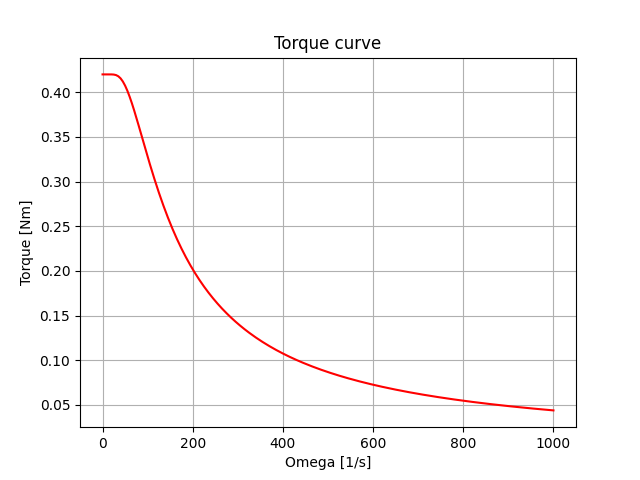
\includegraphics[scale=0.5]{../test/Torque_Curve.png}
    \end{center}
    
\section{Start and Stop speed}

    The starting point of an acceleration curve is the first step starting from standstill. If the motor cannot reach the first step before the controller recharges the coils, 
    the motor will end up not working at all. As mentioned, the acceleration of the motor is the main parameter if it comes to start/stop speed. It is defined as following
    \begin{equation}
        \alpha(t) = \alpha_m (1 - e^{-\frac{t}{\tau}}) \quad \alpha_m = \frac{T_S - T_L}{J} \quad T_L < T_S
    \end{equation}

    With $J$ being the inertia moment of the whole construction connected to the motor, $T_L$ being the torque loss and $\alpha_M$ the maximum angluar velocity.
    Using the basic relationships over the integral
    \[
        \omega(t) = \int \alpha(t) \, dt \quad \phi(t) = \int \omega(t) \, dt
    \]
    \begin{equation}
        \phi(t) = \alpha_m (\frac{t^2}{2} - \tau^2 e^{-\frac{t}{\tau}})
    \end{equation}

    Especially for small motors at high voltages, the second term in the brackets can be ignored, as $\tau^2$ approaches 0. Now to get the minium first step time, this distance has to equal the step distance of the motor
    \[
        \frac{2\pi}{n_S} = \alpha_m \frac{t^2}{2}
    \]
    \begin{equation}
        t = \sqrt{\frac{4\pi}{\alpha_m n_S}}
    \end{equation}

    where $n_S$ is the step count of the motor.

\section{Acceleration curve}

    When knowing the start/stop speed, the acceleration curve can be defined as a series:
    \begin{equation}
        t_0 = \sqrt{\frac{4\pi}{\alpha_m n_S}} \quad
        t_{n} = \frac{2\pi}{n_S\omega(t_t)} \quad t_t = \sum_{i = 0}^{n - 1}{t_i}
    \end{equation}
    
    Example curve:
    \begin{center}
        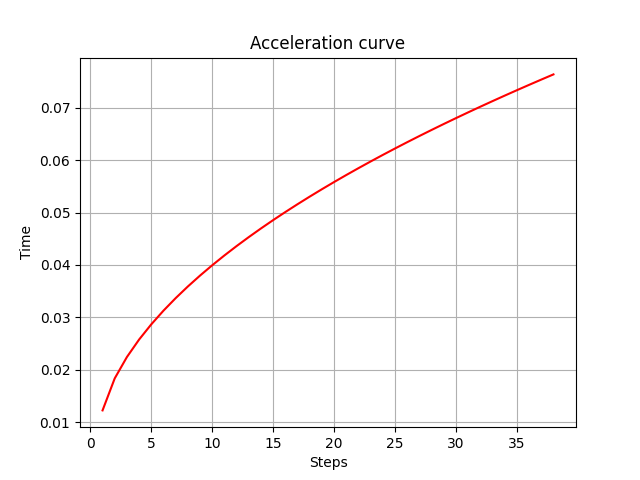
\includegraphics[scale=0.75]{../test/data/Curve1.png}
    \end{center}

\end{document}